For the initial Denial of Service simulation, the network topology is as shown
in Figure \ref{fig:dosNetwork}. This network consists of an attacking traffic
source (shown on the left), a legitimate user traffic source (shown on the
right), and a server (shown on the bottom).

\begin{figure}[H]
	\centering
	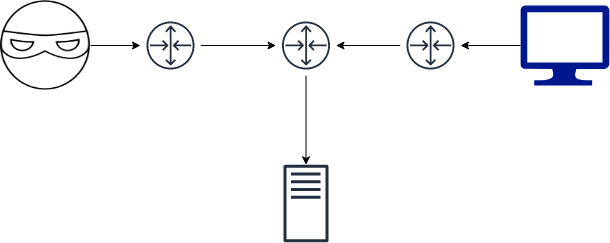
\includegraphics[width=0.8\textwidth]{images/DoS}
	\caption{Denial of Service Network Topology}
	\label{fig:dosNetwork}
\end{figure}

This topology is implemented using the Mininet Python API. Each of the traffic
sources is implemented as a "host", and each switch as a "switch". The links
between each node in the network must be defined. The completed topology
configuration is as follows:

\begin{lstlisting}[language=python, caption=DoS Simulation Network Topology]
class MyTopo( Topo ):
	"Dos Topology"

	def __init__( self ):
		"Create custom topo"

		# Initialize topology
	        Topo.__init__(self)

	        # Add hosts and switches
	        h1 = self.addHost( 'h1' )
	        h2 = self.addHost( 'h2' )
	        h3 = self.addHost( 'h3' )
	        s1 = self.addSwitch( 's1' )
	        s2 = self.addSwitch( 's2' )
	        s3 = self.addSwitch( 's3' )

	        # Add links
	        self.addLink( h1, s1 )
	        self.addLink( s1, s2 )
	        self.addLink( s2, h3 )
	        self.addLink( s2, s3 )
	        self.addLink( s3, h2 )
\end{lstlisting}

\subsection{SYN Flood}

\subsubsection{Attack}

For the SYN Flood, the malicious traffic source launches the attack using the
following "hping" command:

\begin{lstlisting}[language=bash, caption=SYN Flood DoS Command]
$ hping -S -p <TargetPort> --rand-source --flood <TargetIP>
\end{lstlisting}

This command can be broken down as follows:

\begin{itemize}
	\item The -S flag denotes setting the SYN flag for the transmission.
	\item The -p flag sets the destination port number for the transmit
		packet, in this case the target server.
	\item The --rand-source flag sets the IP address to spoofed values for
		each packet that is transmit.
	\item The "--flood" flag sends packets as fast as is possible.

\end{itemize}


\subsubsection{Mitigation}

\subsection {ICMP Flood DoS Attack}

\subsubsection{Attack}

For the ICMP Flood, the malicious traffic source launches the attack using the
following "ping" command:

\begin{lstlisting}[language=bash, caption=ICMP Flood DoS Command]
$ sudo ping -f -l 100000000000000 -s 1500
\end{lstlisting}

This command can be broken down as follows:

\begin{itemize}
	\item The -f flag denotes a flood, as such the tool outputs
		"ECHO\_REQUEST" packets as fast as is possible.
	\item The -l flag denotes the number of packets to send without waiting
		for a reply. The value associated with this flag is set to an
		arbitrarily high number.
	\item The -s flag denotes the packet size, the value for which can be
		determined by observing the output of the "ifconfig eth0". For
		the DoS network, this value was set to 1500 bytes.
\end{itemize}

\subsubsection{Mitigation}
